% This is the template used for the GIH thesis. It is based on 
% Reed College LaTeX thesis template. Most of the work (Reed template)
% for the document class was done by Sam Noble (SN), as well as this
% template. Later comments etc. by Ben Salzberg (BTS). Additional
% restructuring and APA support by Jess Youngberg (JY).
%
% See http://web.reed.edu/cis/help/latex.html for help. There are a
% great bunch of help pages there, with notes on
% getting started, bibtex, etc. Go there and read it if you're not
% already familiar with LaTeX.
%
% Any line that starts with a percent symbol is a comment.
% They won't show up in the document, and are useful for notes
% to yourself and explaining commands.
% Commenting also removes a line from the document;
% very handy for troubleshooting problems. -BTS

% The template was updated by Daniel Hammarström to fit GIH
% requirements. Additional code was borrowed from the 
% Stockholm University (Andreas Solders 2011) template.

% The template was forked from the thesisdown package (CII updates)

%%
%% Preamble
%%
% \documentclass{<something>} must begin each LaTeX document
\documentclass[twoside,10pt]{gihclass} %Default style using S5 paper
% Packages are extensions to the basic LaTeX functions. Whatever you
% want to typeset, there is probably a package out there for it.
% Chemistry (chemtex), screenplays, you name it.
% Check out CTAN to see: http://www.ctan.org/
%%
\usepackage{graphicx,latexsym}
\usepackage{amsmath}
\usepackage{amssymb,amsthm}
\usepackage{longtable,booktabs,setspace}
\usepackage{chemarr} %% Useful for one reaction arrow, useless if you're not a chem major
\usepackage[hyphens]{url}
% Added by CII
\usepackage{hyperref,xcolor}
\hypersetup{
    colorlinks = false,
    pdfborder={0 0 0}
}
\usepackage{lmodern}
\usepackage{float}
\floatplacement{figure}{H}
% End of CII addition
\usepackage{rotating}

% Next line commented out by CII
%%% \usepackage{natbib}
% Comment out the natbib line above and uncomment the following two lines to use the new
% biblatex-chicago style, for Chicago A. Also make some changes at the end where the
% bibliography is included.
%\usepackage{biblatex-chicago}
%\bibliography{thesis}


% Added by CII (Thanks, Hadley!)
% Use ref for internal links
\renewcommand{\hyperref}[2][???]{\autoref{#1}}
\def\chapterautorefname{Chapter}
\def\sectionautorefname{Section}
\def\subsectionautorefname{Subsection}
% End of CII addition

% Added by CII
\usepackage{caption}
\captionsetup{width=5in}
% End of CII addition


% \usepackage{times} % other fonts are available like times, bookman, charter, palatino

% Syntax highlighting #22
  \usepackage{color}
  \usepackage{fancyvrb}
  \newcommand{\VerbBar}{|}
  \newcommand{\VERB}{\Verb[commandchars=\\\{\}]}
  \DefineVerbatimEnvironment{Highlighting}{Verbatim}{commandchars=\\\{\}}
  % Add ',fontsize=\small' for more characters per line
  \usepackage{framed}
  \definecolor{shadecolor}{RGB}{248,248,248}
  \newenvironment{Shaded}{\begin{snugshade}}{\end{snugshade}}
  \newcommand{\AlertTok}[1]{\textcolor[rgb]{0.94,0.16,0.16}{#1}}
  \newcommand{\AnnotationTok}[1]{\textcolor[rgb]{0.56,0.35,0.01}{\textbf{\textit{#1}}}}
  \newcommand{\AttributeTok}[1]{\textcolor[rgb]{0.77,0.63,0.00}{#1}}
  \newcommand{\BaseNTok}[1]{\textcolor[rgb]{0.00,0.00,0.81}{#1}}
  \newcommand{\BuiltInTok}[1]{#1}
  \newcommand{\CharTok}[1]{\textcolor[rgb]{0.31,0.60,0.02}{#1}}
  \newcommand{\CommentTok}[1]{\textcolor[rgb]{0.56,0.35,0.01}{\textit{#1}}}
  \newcommand{\CommentVarTok}[1]{\textcolor[rgb]{0.56,0.35,0.01}{\textbf{\textit{#1}}}}
  \newcommand{\ConstantTok}[1]{\textcolor[rgb]{0.00,0.00,0.00}{#1}}
  \newcommand{\ControlFlowTok}[1]{\textcolor[rgb]{0.13,0.29,0.53}{\textbf{#1}}}
  \newcommand{\DataTypeTok}[1]{\textcolor[rgb]{0.13,0.29,0.53}{#1}}
  \newcommand{\DecValTok}[1]{\textcolor[rgb]{0.00,0.00,0.81}{#1}}
  \newcommand{\DocumentationTok}[1]{\textcolor[rgb]{0.56,0.35,0.01}{\textbf{\textit{#1}}}}
  \newcommand{\ErrorTok}[1]{\textcolor[rgb]{0.64,0.00,0.00}{\textbf{#1}}}
  \newcommand{\ExtensionTok}[1]{#1}
  \newcommand{\FloatTok}[1]{\textcolor[rgb]{0.00,0.00,0.81}{#1}}
  \newcommand{\FunctionTok}[1]{\textcolor[rgb]{0.00,0.00,0.00}{#1}}
  \newcommand{\ImportTok}[1]{#1}
  \newcommand{\InformationTok}[1]{\textcolor[rgb]{0.56,0.35,0.01}{\textbf{\textit{#1}}}}
  \newcommand{\KeywordTok}[1]{\textcolor[rgb]{0.13,0.29,0.53}{\textbf{#1}}}
  \newcommand{\NormalTok}[1]{#1}
  \newcommand{\OperatorTok}[1]{\textcolor[rgb]{0.81,0.36,0.00}{\textbf{#1}}}
  \newcommand{\OtherTok}[1]{\textcolor[rgb]{0.56,0.35,0.01}{#1}}
  \newcommand{\PreprocessorTok}[1]{\textcolor[rgb]{0.56,0.35,0.01}{\textit{#1}}}
  \newcommand{\RegionMarkerTok}[1]{#1}
  \newcommand{\SpecialCharTok}[1]{\textcolor[rgb]{0.00,0.00,0.00}{#1}}
  \newcommand{\SpecialStringTok}[1]{\textcolor[rgb]{0.31,0.60,0.02}{#1}}
  \newcommand{\StringTok}[1]{\textcolor[rgb]{0.31,0.60,0.02}{#1}}
  \newcommand{\VariableTok}[1]{\textcolor[rgb]{0.00,0.00,0.00}{#1}}
  \newcommand{\VerbatimStringTok}[1]{\textcolor[rgb]{0.31,0.60,0.02}{#1}}
  \newcommand{\WarningTok}[1]{\textcolor[rgb]{0.56,0.35,0.01}{\textbf{\textit{#1}}}}

% To pass between YAML and LaTeX the dollar signs are added by CII

% New variables 2019-02-06 GIH copyright info 
\isbn{Provided by the library} 
\place{Stockholm}
\printeby{Printer service, Stockholm, 2019}
\coverinfo{}
\year{2019}



\title{Determinants of intra-individual variation in adaptability to resistance training of different volumes with special reference to skeletal muscle phenotypes}
\author{Daniel Hammarström}
% The month and year that you submit your FINAL draft TO THE LIBRARY (May or December)
\date{May 20xx}


%If you have two advisors for some reason, you can use the following
% Uncommented out by CII
\sernr{999}
% End of CII addition
%%% Remember to use the correct department!

% if you're writing a thesis in an interdisciplinary major,
% uncomment the line below and change the text as appropriate.
% check the Senior Handbook if unsure.
%\thedivisionof{The Established Interdisciplinary Committee for}
% if you want the approval page to say "Approved for the Committee",
% uncomment the next line
%\approvedforthe{Committee}

% Added by CII
%%% Copied from knitr
%% maxwidth is the original width if it's less than linewidth
%% otherwise use linewidth (to make sure the graphics do not exceed the margin)
\makeatletter
\def\maxwidth{ %
  \ifdim\Gin@nat@width>\linewidth
    \linewidth
  \else
    \Gin@nat@width
  \fi
}
\makeatother

\renewcommand{\contentsname}{Table of Contents}
% End of CII addition

\setlength{\parskip}{0pt}

% Added by CII

\providecommand{\tightlist}{%
  \setlength{\itemsep}{0pt}\setlength{\parskip}{0pt}}




\Dedication{
You can have a dedication here if you wish.
}

\Preface{

}

\Abstract{
The preface pretty much says it all.

\par

Second paragraph of abstract starts here.
}

\Listofpapers{
\begin{enumerate}
\def\labelenumi{\Roman{enumi}.}
\item
  \textbf{Hammarström D}, Øfsteng S, Koll L, Hanestadhaugen M, Hollan I, Apró W, Blomstrand E, Rønnestad B, Ellefsen S Benefits of higher resistance-training volume are related to ribosome biogenesis. The \emph{Journal of physiology}. 2020;598(3):543-65.
\item
  Khan Y, \textbf{Hammarström D}, Rønnestad B, Ellefsen S, Ahmad R Increased biological relevance of transcriptome analyses in human skeletal muscle using a model-specific pipeline. \emph{Submitted.}
\item
  \textbf{Hammarström D}, Øfsteng S, Koll L, Jacobsen N, Flobergseter K, Rønnestad B, Ellefsen S Ribosome accumulation during early phase resistance training. \emph{Manuscript}
\item
  \textbf{Hammarström D}, Ellefsen S. generefer: A R package for unbiased selection of reference genes for qPCR in repeated measures designs. \emph{Manuscript}
\end{enumerate}
}


	\usepackage{lettrine} \usepackage{booktabs} \usepackage{longtable} \usepackage{array} \usepackage{multirow} \usepackage{wrapfig} \usepackage{float} \usepackage{colortbl} \usepackage{pdflscape} \usepackage{tabu} \usepackage{threeparttable} \usepackage{threeparttablex} \usepackage[normalem]{ulem} \usepackage{makecell}
	\usepackage{booktabs}
\usepackage{longtable}
\usepackage{array}
\usepackage{multirow}
\usepackage{wrapfig}
\usepackage{float}
\usepackage{colortbl}
\usepackage{pdflscape}
\usepackage{tabu}
\usepackage{threeparttable}
\usepackage{threeparttablex}
\usepackage[normalem]{ulem}
\usepackage{makecell}
% End of CII addition
%%
%% End Preamble
%%
%
\begin{document}




% Everything below added by CII


\frontmatter % this stuff will be roman-numbered
% \pagestyle{empty} % this removes page numbers from the frontmatter
  \maketitle
  \begin{dedication}
  \topskip0pt
\vspace*{\fill}
 You can have a dedication here if you wish.
\vspace*{\fill}
  \end{dedication}
\begin{defence}
    THESIS FOR DOCTORAL DEGREE (Ph.D.)\\
    ~\\
    ~\\
    \textbf{The title of your thesis}\\
    ~\\
    by\\
    \textbf{Your name}\\
    ~\\
    ~\\
    Thesis for Philosophy of Doctoral Degree in Sport Sciences, at The Swedish School of Sport and Health Sciences (GIH), which, according to the decision of the dean, will be publicly defended on \emph{DATE}. The thesis defense will be held at the auditorium at The Swedish School of Sport and Health Sciences (GIH), Stockholm.\\
    ~\\
    ~\\
    \textbf{Opponent}\\
    Profesor \ldots.\\
    ~\\
    \textbf{Principal supervisor}\\
    Profesor\ldots{}\\
    ~\\
    \textbf{Co-supervisor(s)}\\
    -Professor\ldots{}\\
    -Professor\ldots{}\\
    -Professor\ldots{}\\
    ~\\
    \textbf{Examination board}\\
    -Associate professor\ldots{}\\
    -Professor \ldots{}\\
    -Professor \ldots{}
  \end{defence}

  \begin{abstract}
    The preface pretty much says it all.
    
    \par
    
    Second paragraph of abstract starts here.
  \end{abstract}
  \begin{listofpapers}
    \begin{enumerate}
    \def\labelenumi{\Roman{enumi}.}
    \item
      \textbf{Hammarström D}, Øfsteng S, Koll L, Hanestadhaugen M, Hollan I, Apró W, Blomstrand E, Rønnestad B, Ellefsen S Benefits of higher resistance-training volume are related to ribosome biogenesis. The \emph{Journal of physiology}. 2020;598(3):543-65.
    \item
      Khan Y, \textbf{Hammarström D}, Rønnestad B, Ellefsen S, Ahmad R Increased biological relevance of transcriptome analyses in human skeletal muscle using a model-specific pipeline. \emph{Submitted.}
    \item
      \textbf{Hammarström D}, Øfsteng S, Koll L, Jacobsen N, Flobergseter K, Rønnestad B, Ellefsen S Ribosome accumulation during early phase resistance training. \emph{Manuscript}
    \item
      \textbf{Hammarström D}, Ellefsen S. generefer: A R package for unbiased selection of reference genes for qPCR in repeated measures designs. \emph{Manuscript}
    \end{enumerate}
  \end{listofpapers}

  \hypersetup{linkcolor=black}
  \setcounter{tocdepth}{2}
  \tableofcontents

  \listoftables

  \listoffigures




\mainmatter % here the regular arabic numbering starts
\pagestyle{fancyplain} % turns page numbering back on

\setcounter{DefaultLines}{3}

\hypertarget{introduction}{%
\chapter{Introduction}\label{introduction}}

\lettrine{S}keletal muscle health is essential for physical independence. In a lifespan perspective, measures of muscle mass and/or strength are inversely associated with mortality
(1--6)
and disability
(7).
Besides adverse associations between of low muscle mass and strength and clinical conditions, muscle weakness also accounts for increased health care costs in patient populations
(8,9).
The intercept between muscle mass, muscle function and health status is interrelated with variables such as age and primary illness or injury
(10).
This highlights that interventions designed to increase muscle mass and strength are likely to prevent adverse health outcomes across the lifespan. A higher level of muscle mass and functional capacity would counteract the effects of muscle loss due to illness, age or inactivity.

Although a large degree of the observed variations in lean mass and strength are attributed to genetic components
(11,12),
environmental factors also contribute, leaving a window of opportunity to increase muscle mass and functional capacity. Among factors affecting muscle mass and functioning are nutrition and pharmacological agents. However, physical activity and specifically systematic resistance training of sufficient volume, intensity and frequency provides a stimulus that promote morphological and functional changes to the human neuromuscular system without adverse side-effects. Irrespective of age, resistance training generally leads to increased muscle mass and strength
(13,14)
and is considered safe when performed in a well organized manner
(14,15).

Resistance training can be modulated indefinitely through combined variations of training variables such as frequency, intensity and volume
(16,17).
Well designed training prescriptions should incorporate information about the current state and goals of the trainee to maximize the potential outcome of the training program
(16--18).
Training volume has received particular attention in the scientific community for many reasons. Evidence suggests that exercise volume affects selected molecular determinants of muscle hypertrophy in a dose-dependent manner
(19--21).
Such effects are believed to facilitate long-term training effects as training programs with higher volume generally result in higher gains in muscle mass and strength with little evidence of differences between age groups or participants with different training backgrounds
(22--24). \\
A consequence of a more extensive training program is the increased time required to complete such a program. As time constraints has been reported as a limiting factor for engaging in physical activity
(25)
some merit can be given to arguments against guidlines suggesting higher volume in resistance training prescription
(18,26).
From an individual perspective, training prescription that balances time-requirement with efficacy presumably increases the likelihood of participation in physical activity (25).
From a more general perspective, increased knowledge about mechanisms governing responses to physical training could improve training prescription also for individuals and populations that experience attenuated benefit of resistance training
(27).
The overreaching goal of the present thesis is to contribute to understanding individualized training loads. To this end, training volume was used to study the effects of variable training stimulus in within-participant models of exercise-training.

\hypertarget{background}{%
\chapter{Background}\label{background}}

\hypertarget{exercise-training-variables-affecting-training-outcomes}{%
\section{Exercise training variables affecting training outcomes}\label{exercise-training-variables-affecting-training-outcomes}}

\hypertarget{exercise-volume}{%
\section{Exercise volume}\label{exercise-volume}}

\hypertarget{meta-analysis-of-exercise-volume}{%
\subsection{Meta-analysis of exercise volume}\label{meta-analysis-of-exercise-volume}}

\hypertarget{molecular-determinants-of-training-induced-muscle-hypertrophy}{%
\section{Molecular determinants of training-induced muscle hypertrophy}\label{molecular-determinants-of-training-induced-muscle-hypertrophy}}

\hypertarget{protein-synthesis}{%
\subsection{Protein synthesis}\label{protein-synthesis}}
\begin{figure}
\centering
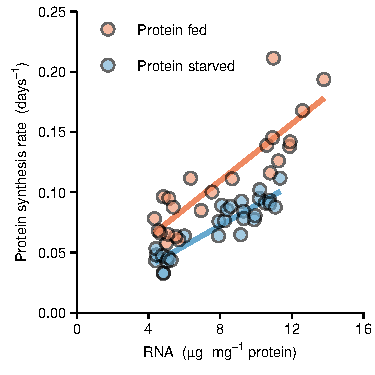
\includegraphics{thesis_files/figure-latex/Millward1973-1.pdf}
\caption{\label{fig:Millward1973}Data from Millward et al.~1973. Group A were fed a diet containing protein, group B were starved or fed a diet not containing protein.}
\end{figure}
\hypertarget{the-mammalian-target-of-rapamycin-mtor-and-translational-efficiency}{%
\subsection{The mammalian target of rapamycin (mTOR) and translational efficiency}\label{the-mammalian-target-of-rapamycin-mtor-and-translational-efficiency}}

The mammalian target of rapamycin (mTOR) is a large serine-threonine protein kinase wich in complex with oyher regulatory proteins forms a signaling hub responsible for responses to environmental cues such as nutrients and mechanical stress.

mTOR has several phosphorylation sites

Phosphorylation of Ser2448 is mediated by S6K1 to reduce mTOR activity in a negative feedback loop .

Ser2448 is phosphorylated by S6K1, changes in nutrient avaliability modifies S6K1 and Ser2448, Ser2448 phosphorylation is abolished when S6K1 is depleted

When the C-terminal is deleted, mTOR gets constitutively active

\hypertarget{ribsome-biogenesis}{%
\subsection{Ribsome biogenesis}\label{ribsome-biogenesis}}

\hypertarget{transcription-of-ribsomal-rna-rrna}{%
\subsubsection{Transcription of ribsomal RNA (rRNA)}\label{transcription-of-ribsomal-rna-rrna}}

\hypertarget{transcriptional-activity-related-to-muscle-hypertrophy}{%
\section{Transcriptional activity related to muscle hypertrophy}\label{transcriptional-activity-related-to-muscle-hypertrophy}}

\hypertarget{methods-for-studying-transcriptional-regulation}{%
\subsection{Methods for studying transcriptional regulation}\label{methods-for-studying-transcriptional-regulation}}

\hypertarget{aims}{%
\chapter{Aims}\label{aims}}

The primary aim of this thesis was to relate the adaptive response to resistance training with low- and moderate-volume to skeletal-muscle characteristics in previously untrained individuals. The key question was whether manipulation of exercise-volume will have diverse effects in different individuals related to muscular intrinsic characteristics. A further aim was to characterize exercise-volume dependence and time course profiles of molecular mechanism thought to control resistance training-induced muscle growth. Based on these aims, the objectives of the present thesis were;
\begin{itemize}
\tightlist
\item
  to relate skeletal muscle and systemic characteristics to benefit of moderate- compared to low-volume resistance training;
\item
  To determine volume-dependence in molecular networks related to muscle growth and remodelling in response to mechanical stress
\item
  To determine a time course of markers related to ribosome biogenesis in the early phase of resistance training.
\end{itemize}
\hypertarget{methods}{%
\chapter{Methods}\label{methods}}

\hypertarget{study-participants-protocols-and-training-interventions}{%
\section{Study participants, protocols and training interventions}\label{study-participants-protocols-and-training-interventions}}

Study I was designed to examine effects of low- and moderate-volume on responses to acute exercise and long-term training within participants. Forty-one healthy individuals were recruited and 34 of these completed at least 85\% of the prescribed sessions and were thus included in subsequent data analyses. Reasons for not completing the trial included injury not related to the study (\emph{n =} 1), pain or discomfort during exercises (\emph{n = }5) and non-adherence to the study protocol. There were no differences in characteristics between participants included in or excluded from data analysis in Study I. Study II was designed to study the effects of resistance training \emph{per se} and effects of variable volume on selected markers related to ribosome biogenesis. Participants were therefore recruited to a training group (\emph{n =} 11) and a non-training control group (\emph{n =} 8). Eligible for participation were young (Study I 18-40; Study II 18-35), non-smoking men and women. Exclusion criteria included a training history of more than one weekly session during the last 12 (Study I) or six (Study II) months leading up to the study. Participants were also screened for intolerance to local anesthetic, current or previous injuries affecting their ability to perform resistance training, self-reported symptoms or history of disease, intake of medication or supplements with known effects on adaptations to training. Participant characteristics for both studies are shown in \ref{tab:characteristics-table}.
\begin{table}

\caption{\label{tab:characteristics-table}Participant characteristics}
\centering
\fontsize{7}{9}\selectfont
\begin{tabular}[t]{llllllll}
\toprule
  &   & Sex & Age (years) & Stature
(cm) & Mass (kg) & Fat mass (\%) & Lean mass (\%)\\
\midrule
 &  & Female & 22.0 (1.3) & 168 (7) & 64.4 (10.4) & 34.1 (5.6) & 64.3 (6.2)\\
\cmidrule{3-8}
 & \multirow{-2}{*}{\raggedright\arraybackslash Included} & Male & 23.6 (4.1) & 183 (6) & 75.8 (10.7) & 20.4 (6.0) & 79.3 (5.0)\\
\cmidrule{2-8}
 &  & Female & 22.9 (1.6) & 166 (8) & 64.6 (9.7) & 28.8 (8.7) & 68.6 (9.1)\\
\cmidrule{3-8}
\multirow{-4}{*}{\raggedright\arraybackslash Study I} & \multirow{-2}{*}{\raggedright\arraybackslash Excluded} & Male & 24.3 (1.5) & 189 (5) & 88.2 (22.4) & 24.3 (15.3) & 76.8 (12.7)\\
\cmidrule{1-8}
 &  & Female & 23.4 (2.9) & 168 (8) & 64.0 (9.2) & 30.8 (7.1) & 65.5 (6.8)\\
\cmidrule{3-8}
 & \multirow{-2}{*}{\raggedright\arraybackslash Training} & Male & 25.7 (5.8) & 177 (3) & 77.5 (8.0) & 25.3 (3.9) & 71.3 (2.4)\\
\cmidrule{2-8}
 &  & Female & 24.1 (3.5) & 166 (4) & 63.8 (0.6) & 30.5 (6.4) & 66.3 (5.2)\\
\cmidrule{3-8}
\multirow{-4}{*}{\raggedright\arraybackslash Study II} & \multirow{-2}{*}{\raggedright\arraybackslash Control} & Male & 25.5 (5.5) & 182 (5) & 76.5 (7.7) & 18.2 (5.1) & 78.7 (4.2)\\
\bottomrule
\multicolumn{8}{l}{\rule{0pt}{1em}Data are means and (SD)}\\
\end{tabular}
\end{table}
\hypertarget{ethical-considerations}{%
\subsection{Ethical considerations}\label{ethical-considerations}}

Both studies were approved by the local ethics committee Lillehammer University College/Inland Norway University of Applied Sciences and the Norwegian Centre for Research Data. In accordance with the \emph{Declaration of Helsinki}({\textbf{???}}) the studies were pre-registered in publicly accessible databases (Study I, ClinicalTrials.gov Identifier: NCT02179307; Study II, \url{https://osf.io/wa96y}). Participants were informed of the study design, potential risks and sources of discomfort prior to giving their informed consent.

\hypertarget{measures-of-muscle-mass}{%
\section{Measures of muscle mass}\label{measures-of-muscle-mass}}

In Study I muscle mass was measured by magnetic resonance imaging (MRI) and dual energy X-ray absorptiometry (DXA) prior to and after the intervention. Both MRI and DXA measurements were completed during the same visit to the laboratory. Participants were instructed to refrain from strenuous physical activity during the last 48 h leading up to the measurements. The post-training measurements were completed at least 48 h after the last strength testing session. Participants were asked to refrain from food consumption during 2 h leading up to the measurements.

MRI images were obtained from the mid-thigh and analyzed by the same investigator blinded for time (pre- and post-training) and condition (low- and moderate-volume). Multiple images were used to estimate the cross-sectional area of the extensor muscles at the same distance from the knee-joint.

See figure

Dallin et al.~recently estimated the (28)

\hypertarget{muscle-strength-assessments}{%
\section{Muscle strength assessments}\label{muscle-strength-assessments}}

\hypertarget{blood-variables}{%
\section{Blood variables}\label{blood-variables}}

\hypertarget{muscle-tissue-sampling-and-preparations-for-downstream-analyses}{%
\section{Muscle tissue sampling and preparations for downstream analyses}\label{muscle-tissue-sampling-and-preparations-for-downstream-analyses}}

\hypertarget{gene-expression-analysis}{%
\section{Gene expression analysis}\label{gene-expression-analysis}}

\hypertarget{determination-of-protein-abundance}{%
\section{Determination of protein abundance}\label{determination-of-protein-abundance}}

\hypertarget{statistics-and-data-analysis}{%
\section{Statistics and data analysis}\label{statistics-and-data-analysis}}

TO DO:
\begin{itemize}
\tightlist
\item
  For methods discussion, compare product length, efficiencies and ct values in relation to RQI-values. See Fleige 2006 for reference.
\end{itemize}
\hypertarget{gene-expression-analysis-1}{%
\section{Gene expression analysis}\label{gene-expression-analysis-1}}

\hypertarget{normalization}{%
\subsection{Normalization}\label{normalization}}
\begin{itemize}
\tightlist
\item
  An external reference gene was added at a constant amount in Trizol preps
\item
  A normalization factor was used to express relative target gene abundance per-weight tissue.
\item
  In qPCR the linearised expression (effectivety \^{}cq) was used to express the fraction of external reference per total RNA.
\item
  In RNA-seq the external reference gene was sequenced and counts were used to express external RNA as a fraction of total RNA.
\item
  In both cases the normalization factor was calculated as mw * counts.
\end{itemize}
A simulation to see that this is equivalent to tissue used in prep when no measurement errors exists.
\begin{Shaded}
\begin{Highlighting}[]
\KeywordTok{library}\NormalTok{(tidyverse)}

\KeywordTok{expand_grid}\NormalTok{(}\DataTypeTok{mg =} \KeywordTok{seq}\NormalTok{(}\DataTypeTok{from =} \DecValTok{5}\NormalTok{, }\DataTypeTok{to =} \DecValTok{100}\NormalTok{, }\DataTypeTok{by =} \DecValTok{5}\NormalTok{), }
            \DataTypeTok{rna.mg =} \KeywordTok{seq}\NormalTok{(}\DataTypeTok{from =} \DecValTok{250}\NormalTok{, }\DataTypeTok{to =} \DecValTok{600}\NormalTok{, }\DataTypeTok{by =} \DecValTok{25}\NormalTok{),}
            \DataTypeTok{ext =} \FloatTok{0.04}\NormalTok{) }\OperatorTok
\StringTok{  }\KeywordTok{mutate}\NormalTok{(}\DataTypeTok{tot.rna =}\NormalTok{ mg }\OperatorTok{*}\StringTok{ }\NormalTok{rna.mg, }
         \DataTypeTok{ext.frac =}\NormalTok{ ext }\OperatorTok{/}\StringTok{ }\NormalTok{(ext }\OperatorTok{+}\StringTok{ }\NormalTok{tot.rna), }
         \DataTypeTok{mg.inprep =} \DecValTok{1000} \OperatorTok{/}\StringTok{ }\NormalTok{((ext }\OperatorTok{+}\StringTok{ }\NormalTok{tot.rna) }\OperatorTok{/}\StringTok{ }\NormalTok{mg), }
         \DataTypeTok{nf =}\NormalTok{ ext.frac }\OperatorTok{*}\StringTok{ }\NormalTok{mg) }
\end{Highlighting}
\end{Shaded}
\begin{verbatim}
# A tibble: 300 x 7
      mg rna.mg   ext tot.rna  ext.frac mg.inprep        nf
   <dbl>  <dbl> <dbl>   <dbl>     <dbl>     <dbl>     <dbl>
 1     5    250  0.04    1250 0.0000320      4.00 0.000160 
 2     5    275  0.04    1375 0.0000291      3.64 0.000145 
 3     5    300  0.04    1500 0.0000267      3.33 0.000133 
 4     5    325  0.04    1625 0.0000246      3.08 0.000123 
 5     5    350  0.04    1750 0.0000229      2.86 0.000114 
 6     5    375  0.04    1875 0.0000213      2.67 0.000107 
 7     5    400  0.04    2000 0.0000200      2.50 0.000100 
 8     5    425  0.04    2125 0.0000188      2.35 0.0000941
 9     5    450  0.04    2250 0.0000178      2.22 0.0000889
10     5    475  0.04    2375 0.0000168      2.11 0.0000842
# ... with 290 more rows
\end{verbatim}
\begin{Shaded}
\begin{Highlighting}[]
\KeywordTok{expand_grid}\NormalTok{(}\DataTypeTok{mg =} \KeywordTok{seq}\NormalTok{(}\DataTypeTok{from =} \DecValTok{5}\NormalTok{, }\DataTypeTok{to =} \DecValTok{100}\NormalTok{, }\DataTypeTok{by =} \DecValTok{5}\NormalTok{), }
            \DataTypeTok{rna.mg =} \KeywordTok{seq}\NormalTok{(}\DataTypeTok{from =} \DecValTok{50}\NormalTok{, }\DataTypeTok{to =} \DecValTok{600}\NormalTok{, }\DataTypeTok{by =} \DecValTok{25}\NormalTok{),}
            \DataTypeTok{ext =} \FloatTok{0.04}\NormalTok{) }\OperatorTok
\StringTok{  }\KeywordTok{mutate}\NormalTok{(}\DataTypeTok{tot.rna =}\NormalTok{ mg }\OperatorTok{*}\StringTok{ }\NormalTok{rna.mg, }
         \DataTypeTok{ext.frac =}\NormalTok{ ext }\OperatorTok{/}\StringTok{ }\NormalTok{(ext }\OperatorTok{+}\StringTok{ }\NormalTok{tot.rna), }
         \DataTypeTok{mg.inprep =} \DecValTok{1000} \OperatorTok{/}\StringTok{ }\NormalTok{((ext }\OperatorTok{+}\StringTok{ }\NormalTok{tot.rna) }\OperatorTok{/}\StringTok{ }\NormalTok{mg), }
         \DataTypeTok{nf =}\NormalTok{ ext.frac }\OperatorTok{*}\StringTok{ }\NormalTok{mg) }\OperatorTok
\StringTok{         }\KeywordTok{ggplot}\NormalTok{(}\KeywordTok{aes}\NormalTok{(rna.mg, mg.inprep,  }\DataTypeTok{color =}\NormalTok{ mg)) }\OperatorTok{+}\StringTok{ }\KeywordTok{geom_point}\NormalTok{(}\DataTypeTok{size =} \DecValTok{2}\NormalTok{)}
\end{Highlighting}
\end{Shaded}
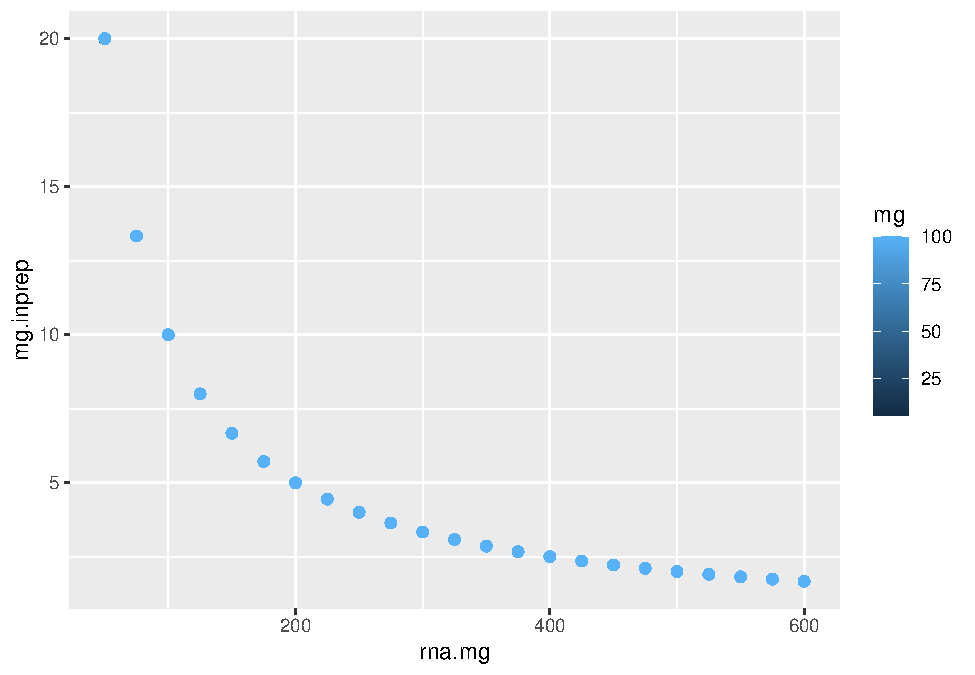
\includegraphics{thesis_files/figure-latex/unnamed-chunk-1-1.pdf}

\hypertarget{training-protocols}{%
\section{Training protocols}\label{training-protocols}}

A full body protocol was used in study I including

\hypertarget{results}{%
\chapter{Results}\label{results}}

\hypertarget{discussion}{%
\chapter{Discussion}\label{discussion}}

\hypertarget{conclusion}{%
\chapter*{Conclusion}\label{conclusion}}
\addcontentsline{toc}{chapter}{Conclusion}

If we don't want Conclusion to have a chapter number next to it, we can add the \texttt{\{-\}} attribute.

\textbf{More info}

And here's some other random info: the first paragraph after a chapter title or section head \emph{shouldn't be} indented, because indents are to tell the reader that you're starting a new paragraph. Since that's obvious after a chapter or section title, proper typesetting doesn't add an indent there.

\backmatter

\hypertarget{references}{%
\chapter*{References}\label{references}}
\addcontentsline{toc}{chapter}{References}

\markboth{References}{References}

\noindent

\setlength{\parindent}{-0.20in}
\setlength{\leftskip}{0.20in}
\setlength{\parskip}{8pt}

\hypertarget{refs}{}
\leavevmode\hypertarget{ref-RN2512}{}%
1. Li R, Xia J, Zhang XI, Gathirua-Mwangi WG, Guo J, Li Y, et al. Associations of muscle mass and strength with all-cause mortality among us older adults. Medicine and science in sports and exercise {[}Internet{]}. 2018;50(3):458--67.

\leavevmode\hypertarget{ref-RN2513}{}%
2. Fukasawa H, Kaneko M, Niwa H, Matsuyama T, Yasuda H, Kumagai H, et al. Lower thigh muscle mass is associated with all-cause and cardiovascular mortality in elderly hemodialysis patients. European Journal of Clinical Nutrition {[}Internet{]}. 2017;71(1):64--9.

\leavevmode\hypertarget{ref-RN2514}{}%
3. Miyake H, Kanazawa I, Tanaka KI, Sugimoto T. Low skeletal muscle mass is associated with the risk of all-cause mortality in patients with type 2 diabetes mellitus. Ther Adv Endocrinol Metab {[}Internet{]}. 2019;10:2042018819842971.

\leavevmode\hypertarget{ref-RN2376}{}%
4. Ruiz JR, Sui X, Lobelo F, Morrow J James R., Jackson AW, Sjöström M, et al. Association between muscular strength and mortality in men: Prospective cohort study. BMJ (Clinical research ed) {[}Internet{]}. 2008;337(7661):a439--9.

\leavevmode\hypertarget{ref-RN2515}{}%
5. Szulc P, Munoz F, Marchand F, Chapurlat R, Delmas PD. Rapid loss of appendicular skeletal muscle mass is associated with higher all-cause mortality in older men: The prospective minos study. Am J Clin Nutr {[}Internet{]}. 2010;91(5):1227--36.

\leavevmode\hypertarget{ref-RN2516}{}%
6. Abramowitz MK, Hall CB, Amodu A, Sharma D, Androga L, Hawkins M. Muscle mass, bmi, and mortality among adults in the united states: A population-based cohort study. PLoS One. 2018;13(4):e0194697.

\leavevmode\hypertarget{ref-RN2517}{}%
7. Janssen I, Heymsfield SB, Ross R. Low relative skeletal muscle mass (sarcopenia) in older persons is associated with functional impairment and physical disability. J Am Geriatr Soc {[}Internet{]}. 2002;50(5):889--96.

\leavevmode\hypertarget{ref-RN2532}{}%
8. Sousa AS, Guerra RS, Fonseca I, Pichel F, Ferreira S, Amaral TF. Financial impact of sarcopenia on hospitalization costs. Eur J Clin Nutr {[}Internet{]}. 2016;70(9):1046--51.

\leavevmode\hypertarget{ref-RN2184}{}%
9. Pinedo-Villanueva R, Westbury LD, Syddall HE, Sanchez-Santos MT, Dennison EM, Robinson SM, et al. Health care costs associated with muscle weakness: A uk population-based estimate. Calcif Tissue Int {[}Internet{]}. 2019;104(2):137--44.

\leavevmode\hypertarget{ref-RN763}{}%
10. Wolfe RR. The underappreciated role of muscle in health and disease. Am J Clin Nutr {[}Internet{]}. 2006;84(3):475--82.

\leavevmode\hypertarget{ref-RN2526}{}%
11. Arden NK, Spector TD. Genetic influences on muscle strength, lean body mass, and bone mineral density: A twin study. Journal of Bone and Mineral Research {[}Internet{]}. 1997;12(12):2076--81.

\leavevmode\hypertarget{ref-RN2527}{}%
12. Roth SM. Genetic aspects of skeletal muscle strength and mass with relevance to sarcopenia. BoneKEy reports {[}Internet{]}. 2012;1:58--8.

\leavevmode\hypertarget{ref-RN1741}{}%
13. Ahtiainen JP, Walker S, Peltonen H, Holviala J, Sillanpaa E, Karavirta L, et al. Heterogeneity in resistance training-induced muscle strength and mass responses in men and women of different ages. Age (Dordr) {[}Internet{]}. 2016;38(1):10.

\leavevmode\hypertarget{ref-RN2534}{}%
14. Grgic J, Garofolini A, Orazem J, Sabol F, Schoenfeld BJ, Pedisic Z. Effects of resistance training on muscle size and strength in very elderly adults: A systematic review and meta-analysis of randomized controlled trials. Sports Med {[}Internet{]}. 2020;

\leavevmode\hypertarget{ref-RN2536}{}%
15. Faigenbaum AD, Myer GD. Resistance training among young athletes: Safety, efficacy and injury prevention effects. British Journal of Sports Medicine {[}Internet{]}. 2010;44(1):56.

\leavevmode\hypertarget{ref-RN1}{}%
16. Ratamess N, Alvar BA, Evetoch TK, Housh TJ, Kibler B, Kraemer WJ, et al. American college of sports medicine position stand. Progression models in resistance training for healthy adults. Med Sci Sports Exerc {[}Internet{]}. 2009;41(3):687--708.

\leavevmode\hypertarget{ref-RN798}{}%
17. Bird SP, Tarpenning KM, Marino FE. Designing resistance training programmes to enhance muscular fitness: A review of the acute programme variables. Sports Med {[}Internet{]}. 2005;35(10):841--51.

\leavevmode\hypertarget{ref-RN2538}{}%
18. Feigenbaum MS, Pollock ML. Prescription of resistance training for health and disease. Med Sci Sports Exerc. 1999;31(1):38--45.

\leavevmode\hypertarget{ref-RN791}{}%
19. Burd NA, Holwerda AM, Selby KC, West DW, Staples AW, Cain NE, et al. Resistance exercise volume affects myofibrillar protein synthesis and anabolic signalling molecule phosphorylation in young men. J Physiol {[}Internet{]}. 2010;588(Pt 16):3119--30.

\leavevmode\hypertarget{ref-RN784}{}%
20. Terzis G, Spengos K, Mascher H, Georgiadis G, Manta P, Blomstrand E. The degree of p70 s6k and s6 phosphorylation in human skeletal muscle in response to resistance exercise depends on the training volume. Eur J Appl Physiol {[}Internet{]}. 2010;110(4):835--43.

\leavevmode\hypertarget{ref-RN1837}{}%
21. Ahtiainen JP, Walker S, Silvennoinen M, Kyrolainen H, Nindl BC, Hakkinen K, et al. Exercise type and volume alter signaling pathways regulating skeletal muscle glucose uptake and protein synthesis. Eur J Appl Physiol. 2015;115(9):1835--45.

\leavevmode\hypertarget{ref-RN793}{}%
22. Krieger JW. Single versus multiple sets of resistance exercise: A meta-regression. J Strength Cond Res {[}Internet{]}. 2009;23(6):1890--901.

\leavevmode\hypertarget{ref-RN789}{}%
23. Krieger JW. Single vs. Multiple sets of resistance exercise for muscle hypertrophy: A meta-analysis. J Strength Cond Res {[}Internet{]}. 2010;24(4):1150--9.

\leavevmode\hypertarget{ref-RN1767}{}%
24. Schoenfeld BJ, Ogborn D, Krieger JW. Dose-response relationship between weekly resistance training volume and increases in muscle mass: A systematic review and meta-analysis. J Sports Sci {[}Internet{]}. 2016;1--10.

\leavevmode\hypertarget{ref-RN2063}{}%
25. Choi J, Lee M, Lee JK, Kang D, Choi JY. Correlates associated with participation in physical activity among adults: A systematic review of reviews and update. BMC Public Health {[}Internet{]}. 2017;17(1):356.

\leavevmode\hypertarget{ref-RN794}{}%
26. Carpinelli RN, Otto RM. Strength training. Single versus multiple sets. Sports Med {[}Internet{]}. 1998;26(2):73--84.

\leavevmode\hypertarget{ref-RN2547}{}%
27. Pickering C, Kiely J. Do non-responders to exercise exist---and if so, what should we do about them? Sports Medicine {[}Internet{]}. 2019;49(1):1--7.

\leavevmode\hypertarget{ref-RN2541}{}%
28. Tavoian D, Ampomah K, Amano S, Law TD, Clark BC. Changes in dxa-derived lean mass and mri-derived cross-sectional area of the thigh are modestly associated. Scientific Reports {[}Internet{]}. 2019;9(1):10028.


% Index?

\end{document}
